\documentclass[11pt,English]{article}
\usepackage[utf8]{inputenc}
\usepackage{amsmath}
\usepackage[bottom]{footmisc}

% Keywords command
\providecommand{\keywords}[1]
{
  \small	
  \-\ \-\ \-\ \textbf{\textit{Keywords --}} #1
}

% Plot set up --Thomas--
\usepackage{pgfplots}
\pgfplotsset{compat=1.16,scale=1.25}

\pgfplotsset{
    vector/.style={
        % Axis Line setup
        axis lines=center,
        axis line style={latex-latex},
        % View Set up, to rotate the graph
        view={0}{90},
    }
}





% Slides 
% 
% 1) Authors names and affiliations
% 2) Title abstract keywords
% 3) 147 why its important
%
% History
%
% http://mathshistory.st-andrews.ac.uk/Biographies/Green.html
%
%
%
% Example I
% - Apex Calc III - example "Confirming Green's Theorem" pg. 875
%     https://www.apexcalculus.com/downloads
%
%
%
%
% Example II
%
% 
% https://brilliant.org/wiki/greens-theorem/
%https://www.khanacademy.org/math/multivariable-calculus/greens-theorem-and-stokes-theorem/greens-theorem-articles/a/greens-theorem-examples
%
%

\title{
Green's Theorem\\
    \large Historical Origins and Analytical Applications\\
    \small MATH 147 Final Project\\
    \small University of Kansas, Dept. of Mathematics
}
\author{
    Atkins, Thomas\\
    \texttt{thomas.atkins@ku.edu}
    \and
    Mills, Garrett\\
    \texttt{glmdev@ku.edu}
    \and
    Weng, QiTao\\
    \texttt{wengqt@ku.edu}
}
\date{December 2019}

\begin{document}

\maketitle
\begin{abstract}
    In which the authors investigate the historical origins and several mathematical applications of the commonly known Green's theorem. Discovered by George Green in the late 1820s, this theorem provides a relationship between the line integral of a particular curve and the surface integral of its enclosed region. Green's theorem is closely related to the divergence theorem, and is simply a specific case of the more general Stoke's theorem. Beyond basic applications to flux and surface integrals, Green's theorem can be reverse applied to calculate difficult-to-evaluate area calculations. It also plays an integral role (pun intended) in the proof of other important theorems such as Cauchy's.
\end{abstract}

\keywords{Green, Stoke, integration, vector calculus}

\section{Introduction}

George Green, the mathematician who would go one to postulate the now famous Green's theorem, was born in July of 1793. As a youth he received only a year of formal schooling when he was 8 years old. While working full time at a mile owned by his father in 1728 he published \emph{An Essay on the Application of Mathematical Analysis to the Theories of Electricity and Magnetism.} In that publication Green would put forth the therm that now bears his name, thought it would be years before anyone would fully appreciate it. The publication of the paper would catch the eye of one Sir Edward Bromhead, who would latter encouraged Green to study Mathematics at Cambridge. He would died before his work would be recognized as the landmark discovery it was.\footnote{"George Green
" University of St Andrews, October 1998, (http://mathshistory.st-andrews.ac.uk/Biographies/Green.html)}



% here is some definitions stuffs
Green's theorem is commonly defined as follows.\footnote{"Section 5-7: Green's Theorem" - Paul Dawkins, Lamar University - 02-22-2019. (http://tutorial.math.lamar.edu/Classes/CalcIII/GreensTheorem.aspx)} Let $C$ be a simple, smooth, closed, positive curve and $D$ the region enclosed by said curve. Assume $P'$, $Q'$ are continuous. Then, the following relationship holds:
$$
\int_C{ P dx + Q dy } = \iint_D{ \left( \frac{\partial Q}{\partial x} - \frac{\partial P}{\partial y} \right) dA }
$$


\section{Verification of Green's Theorem}
Green's theorem is commonly used in applications of vector calculus to other fields of study, particularly physics in the plane. One example of this is calculating the circulation of vector fields along a closed boundary. For our purposes, circulation refers to the magnitude of the vector field that \emph{passes through} or \emph{pushes against} the closed boundary.\footnote{"Vector Calculus: Understanding Circulation and Curl" - Editors of BetterExplained, BetterExplained, Vector Calculus - n.d.} 

% ==== Illustration Image of Circulation Here ====

\begin{figure}[]
    \centering
        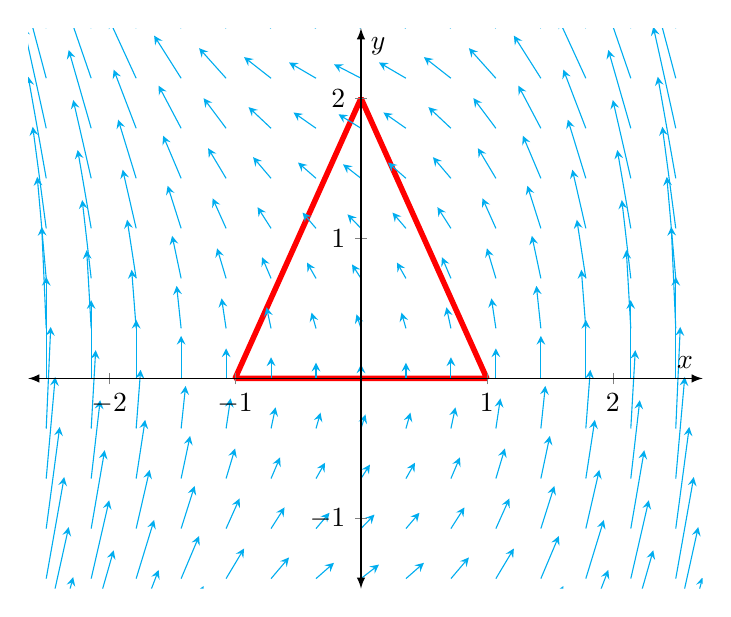
\begin{tikzpicture}
            \begin{axis}[vector,
                title={},
                domain=-2.5:2.5,
                ymin = -1.5,
                ymax = 2.5,
                xlabel=$x$,
                ylabel=$y$,
            ]
                \addplot[
                    patch,
                    patch type=triangle,
                    color = white,
                    line width=2pt,
                    faceted color=red,
                ] 
                    coordinates {
                        (-1,0)
                        (1,0)
                        (0,2)
                    };
                \addplot3[
                    cyan,
                    quiver={
                        u={-y},
                        v={x^2+1},
                        scale arrows=0.1
                    },
                    -stealth,
                    samples=15]
                    {x};
            \end{axis}
        \end{tikzpicture}
    \caption{Illustration of Circulation}
    \label{Circulation}
\end{figure}



Take, for example, the field and boundary pictured above. There is some vector field in the plane, $\vec{E}$, that emanates from some point $P$. Inset in that field is some simple, closed boundary $\partial S$. The circulation of the field $\vec{E}$ with respect to the boundary $\partial S$ is the magnitude $E$ that is incident on $\partial S$. That is, the \emph{amount} of the field that passes through the boundary.

We can verify Green's theorem by calculating the circulation of a vector field manually using line integrals, and using the formula for Green's. Let, for example, our electric field $\vec{E} = \left< -y, x^2+1 \right>$. The boundary, as shown above, is a triangle traversed counter-clockwise, with vertices at $\left( -1, 0 \right)$, $\left( 1, 0 \right)$, and $\left(0, 2\right)$.

\subsection{Using Line Integrals}
We can calculate the circulation using a series of line integrals of parameterizations along the sides of the triangle. Provided that you traverse it counter-clockwise, you can start at any of the vertices. Starting at $\left(-1, 0\right)$, we can use the following parameterizations:
\begin{align}
\vec{r}_1(t) &= \left<2t-1, 0\right> \;\;\;\;\; 0 \leq t \leq 1 \\
\vec{r}_2(t) &= \left<1-t, 2t\right> \;\;\;\;\;\; 0 \leq t \leq 1 \\
\vec{r}_3(t) &= \left<-t, 2-2t\right> \;\;\;\; 0 \leq t \leq 1
\end{align}

The circulation along a single edge (one of the $\vec{r}_i$) can be computed using the following vector line integral:
$$
\Phi_i = \int_{C_i} \vec{E}(\vec{r}_i) \cdot d\vec{r}_i
$$

In each case, the $d\vec{r}_i$ can be computed as $\frac{\partial\vec{r}_i}{\partial t}$. Hence, for our purposes, the various $d\vec{r}_i$ are as follows:
\begin{align}
    \frac{\partial\vec{r}_1}{\partial t} &= \left<2, 0\right> \\
    \frac{\partial\vec{r}_2}{\partial t} &= \left<-1, 2\right> \\
    \frac{\partial\vec{r}_3}{\partial t} &= \left<-1, -2\right>
\end{align}

So we can calculate the various $\Phi_i$ using the formula above. Then, we can find the resultant $\Phi_{net}$ as the sum of the circulations of the individual components.\footnote{This makes an intuitive sense. If you have a bucket with 2 liters of water per second flowing in the top and 1 liter of water per second flowing out the bottom, the total flow of water in the bucket is a gain of 1 liter of water per second ($2 \frac{L}{s} - 1 \frac{L}{s} = 1 \frac{L}{s}$).}

\begin{align*}
    \Phi_1 &= \int_{C_1} \vec{E}(\vec{r}_1) \cdot d\vec{r}_1 \\
    &= \int_0^1 \left<0, (2t-1)^2 +1\right> \cdot \left<2,0\right> dt \\
    &= 0
\end{align*}

\begin{align*}
    \Phi_2 &= \int_{C_2} \vec{E}(\vec{r}_2) \cdot d\vec{r}_2 \\
    &= \int_0^1 \left<-2t, (1-t)^2 +1\right> \cdot \left<-1,2\right> dt \\
    &= \int_0^1 (2t + 2(1-t)^2 +2) \; dt \\
    &= \int_0^1 (2t^2 -2t + 4) \; dt \\
    &= \frac{2}{3}t - t^2 + 4t \vert_0^1 \\
    &= \frac{11}{3}
\end{align*}

\begin{align*}
    \Phi_3 &= \int_{C_3} \vec{E}(\vec{r}_3) \cdot d\vec{r}_3 \\
    &= \int_0^1 \left<2t-2, t^2 +1\right> \cdot \left<-1, -2\right> \\
    &= \int_0^1 -2t-2t^2 \; dt \\
    &= -t^2 -\frac{2}{3}t^3 \mid_0^1 \\
    &= -\frac{5}{3}
\end{align*}

We can then compute the total $\Phi_{net}$ as the sum of the fluxes across the three boundary-components. That is, $\Phi_net = \Phi_1 + \Phi_2 + \Phi_3 = 0 + \frac{11}{3} - \frac{5}{3} = 2$. This result indicates that the flux of the electric field has a magnitude of 2 across the described boundary. Typically, the units for electric flux are Volt-meters ($Vm$).

\subsection{Using Green's Theorem}
As mentioned above, Green's theorem relates the circulation of a vector field over a boundary to the area of the curl of that field over the surface enclosed by the boundary. We can verify the result gained above, then, by calculating the following double-integral:
\begin{align*}
    \int_C \vec{E}(\vec{r}) \cdot d\vec{r} = \iint_D \nabla \times \vec{E} \cdot dA
\end{align*}

We begin by computing the curl of $\vec{E}$ as the virtual cross-product of the nabla-operator against the components of $\vec{E}$:
\begin{align*}
    \nabla \times \vec{E} &=
    \begin{vmatrix}
        \hat{i} & \hat{j} & \hat{k} \\
        \frac{\partial}{\partial x} & \frac{\partial}{\partial y} & \frac{\partial}{\partial z} \\
        -y & x^2 + 1 & 0
    \end{vmatrix} \\
    &= \left<0,0,2x+1\right>
\end{align*}

Now, we can compute the related area by dotting this result with the differential area. Because the boundary lies in the xy-plane, we can take the z-component for our integrand. Thus, the circulation across the boundary can be calculated as such:
\begin{align*}
    \Phi_{net} &= \iint_D \nabla \times \vec{E} \cdot dA \\
    &= \int_0^2 \int_{y/2-1}^{1-y/2} 2x+1 \; dx \; dy \\
    &= \int_0^2 2-y \; dy \\
    &= 2
\end{align*}

Thus, the circulation across the boundary is $2 \; Vm$, which is consistent with the result we found above.

\section{Applications}
Calculating parametric curves using Green's theorem instead of directly computing a line integral can often be much simpler. Calculating the area of a seashell-like spiral:
\begin{align*}
    x(t) = t\cos{t} \\
    y(t) = t\sin{t}  \\
    0<t<2\pi \\
\end{align*}

\end{document}
